\normalfalse \difficiletrue \tdifficilefalse
\correctionfalse

%\UPSTIidClasse{11} % 11 sup, 12 spé
%\newcommand{\UPSTIidClasse}{12}

\exer{Mouvement RR 3D  $\star\star$ \label{C2:08:07}}
\setcounter{numques}{0}
\UPSTIcompetence[2]{C2-08}
\UPSTIcompetence[2]{C2-09}
\index{Compétence C2-08}
\index{Compétence C2-09}
\index{Torseur cinétique}
\index{Torseur dynamique}
\ifcorrection
\else
\textbf{Pas de corrigé pour cet exercice.}
\fi

\ifprof
\else
Soit le mécanisme suivant. On a $\vect{AB}=R\vect{i_1}$ et $\vect{BC}=\ell\vect{i_2}+r\vect{j_2}$. On note $R+\ell=L = \SI{20}{mm}$ et $r=\SI{10}{mm}$. De plus :
\begin{itemize}
\item $G_1=B$ désigne le centre d'inertie de \textbf{1}, on note $m_1$ la masse de \textbf{1} et $\inertie{G_1}{1}$; 
\item $G_2$ désigne le centre d'inertie de \textbf{2} tel que  $\vect{BG_2}=\ell\vect{i_2}$, on note $m_2$ la masse de \textbf{2} et $\inertie{G_2}{2}=\matinertie{A_2}{B_2}{C_2}{0}{0}{0}{\bas{2}}$.
\end{itemize}
\begin{center}
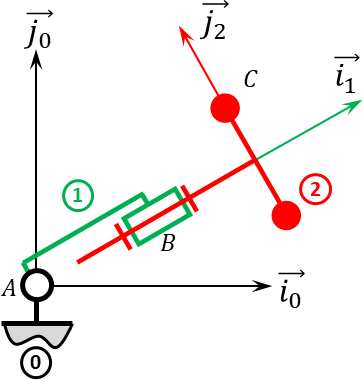
\includegraphics[width=\linewidth]{07_RR3D_01}
\end{center}
\fi

\question{Exprimer le torseur dynamique $\torseurdyn{1}{0}$ en~$B$.}
\ifprof

Par définition, $\torseurdyn{1}{0} = \torseurl{\vectrd{1}{0}}{\vectmd{B}{1}{0}}{B}$.

\textbf{Calculons $\vectrd{1}{0}$}

$\vectrd{1}{0} = m_1\vectg{G_1}{1}{0}=m_1 \vectg{B}{1}{0} $

 \textbf{Calcul de $\vectv{B}{1}{0}$ : }  
$\vectv{B}{1}{0}=\deriv{\vect{AB}}{\rep{0}}$ 
$=\deriv{ R\vi{1}}{\rep{0}}$  
$= R\thetap \vj{1}$.


 \textbf{Calcul de $\vectg{B}{1}{0}$ : }  
$\vectv{B}{1}{0}=\deriv{\vectv{B}{1}{0}}{\rep{0}}$ 
$=\deriv{ R\thetap \vj{1}}{\rep{0}}$  
$=  R\thetapp \vj{1}-R\thetap^2 \vi{1}$.

Au final, $\vectrd{1}{0}= m_1\left(R\thetapp \vj{1}-R\thetap^2 \vi{1}\right)$.
\vspace{.5cm}

\textbf{Calculons $\vectmd{B}{1}{0}$}
$B$ est le centre d'inertie du solide 1; donc 
 d'une part, $\vectmd{B}{1}{0} = \deriv{\vectmc{B}{1}{0} }{\rep{0}}$.
 
 D'autre part, $\vectmc{B}{1}{0} = \inertie{B}{1}\vecto{1}{0}$
 $ =\matinertie{A_1}{B_1}{C_1}{0}{0}{0}{\bas{1}} \thetap \vk{0}$
  $ =C_1 \thetap \vk{0}$.
  
  Par suite, $\vectmd{B}{1}{0} = C_1 \thetapp \vk{0}$.
  
  Au final, 
$\torseurdyn{1}{0} = \torseurl{m_1\left(R\thetapp \vj{1}-R\thetap^2 \vi{1}\right)}{C_1 \thetapp \vk{0}}{B}$


%$= \dfrac{\dd \vect{AB}}{\dd t}$
%$= \dfrac{\dd R\vi{1}}{\dd t}$
%$= R\thetap \vj{1}$.
%
%\noindent \textbf{Calcul de $\vectg{B}{1}{0}$ : }  $\vectg{B}{1}{0}= \dfrac{\dd $\vectv{B}{1}{0}$}{\dd t}$ 
%$= \dfrac{\dd \vect{AB}}{\dd t}$
%$= \dfrac{\dd}{\dd t}$
%$= R\thetap \vj{1}$


\else
\fi

\question{Déterminer $\vectmd{A}{1+2}{0}\cdot \vect{k_0}$}
\ifprof
\else
\fi

\ifprof
\else
\begin{flushright}
\footnotesize{Corrigé  voir \ref{C2:08:07}.}
\end{flushright}%
\fi